
\chapter[Contribution to CO-Optimal Transport]{Contribution to CO-Optimal Transport}

\localtableofcontents*

\chaptermark{\textbf{Contribution to CO-Optimal Transport}}

\section{Introduction}

This chapter is based on the paper \citep{Tran21} and my personal work.


considers a relaxation of the
CO-Optimal Transport problem. OT theory underlies many emerging machine learning
methods nowadays solving a wide range of tasks.
These latter works, however, usually build upon a traditional OT setup with two distributions,
while leaving a more general multi-marginal OT formulation somewhat
unexplored. In this paper, we study the multi-marginal OT (MMOT) problem and unify several
popular OT methods under its umbrella
by promoting structural information on the coupling. We show that incorporating such structural
information into MMOT results in an instance of a difference of convex (DC) programming problem allowing us to solve it numerically.
Despite high computational cost of the latter procedure, the solutions provided by DC optimization are usually as qualitative as
those obtained using currently employed optimization schemes.

Recall that, when the supports of the probability measures lie in the same ground metric space,
it is natural to use the distance defined by the metric
to induce the cost, which leads to the famous Wasserstein distance \citep{Villani03}.
When they do not, one can rely on the idea of Gromov-Hausdorff distance \citep{Gromov81}
and its equivalent reformulations \citep{Gromov99,Kalton99,Burago01},
and adapt them to the setting of metric measure spaces \citep{Gromov99}.
This results in, for example, the celebrated Gromov-Wasserstein distance
\citep{Memoli07,Memoli11,Sturm12}. By construction, the GW distance can only provide
the sample alignment that best preserves the intrinsic geometry of the distributions and,
as such, compares square pairwise relationship matrices.

The CO-Optimal transport (COOT) \citep{Redko20,Chowdhury21b} goes beyond these limits by
simultaneously learning two independent (feature and sample) correspondences,
thus provides greater flexibility over the GW distance in terms of usage and interpretability.
First, it allows to measure similarity between arbitrary-size matrices. An interesting use case is,
for instance, on tabular data, which is usually expressed as a matrix whose rows represent samples
and columns represent features. For the GW distance, the similarity or distance matrix
(or any square matrix derived from the data) must be calculated in advance and
the effect of the individual variables is lost during this computation. By contrast,
COOT can bypass this step as it can use either the tabular data directly or
the similarity matrices as inputs. Second, COOT provides both sample and feature correspondences.
These feature alignments are unique to COOT and prove to be particularly useful,
for example in single-cell multi-omics \citep{Demetci20b}
are also interpretable and allow to recover relations between the features of
two different datasets even when they do not lie in the same space.
COOT has shown superior performance in heterogeneous domain adaptaion \citep{Redko20},

Given a matrix $X \in \bbR^{n \times d}$,
we equip its samples (rows) with the histogram $\mu^s \in \Delta_n$ and features (columns)
with the histogram $\mu^f \in \Delta_d$.
We call the triplet $\bbX = (X, \mu^s, \mu^f)$ a sample-feature (s.f.) space.
For $p \geq 1$, we define the COOT distance between two s.f. spaces
$\bbX = (X, \mu_x^s, \mu_x^f)$ and $\bbY = (Y, \mu_y^s, \mu_y^f)$ as
\begin{align*}
    \coot(\bbX, \bbY) :=
    \inf_{\substack{\pi^s \in U(\mu_x^s, \mu_y^s) \\ \pi^f \in U(\mu_x^f, \mu_y^f)}}
    \sum_{i,j,k,l} (X_{ij} - Y_{kl})^p \pi^s_{ik} \pi^f_{jl}
    = \langle |X - Y|^p, \pi^s \otimes \pi^f \rangle.
\end{align*}
Here, for convenience, we write $|X - Y|^p$ the $4$-D tensor defined by
$(|X - Y|^p)_{i,k,j,l} = (X_{ij} - Y_{kl})^p$. We summarize the versatility of COOT for practical
usage in \Cref{t:comparisons}
\begin{table}[h]
	\centering
		\begin{tabular}{|l|l|}
    \hline
    Distance & Input matrices \\
    \hline
    Frobenius & Same-size matrices \\
    Wasserstein & Matrices with the same number of features (columns) \\
    GW & Square (mostly symmetric) matrices \\
    COOT & Arbitrary-size matrices \\
    \hline
		\end{tabular}
		\caption{but also robust to outliers.
    \label{t:comparisons}}
\end{table}
In the following sections, we will explore some aspects of COOT.

%%%%%%%%%%%%%%%%%%%%%%%%%%%%%%%%%%%%%%
\section{Three shades of discrete Co-Optimal Transport}
%%%%%%%%%%%%%%%%%%%%%%%%%%%%%%%%%%%%%%

\subsection{Co-Optimal Transport as lower bound of GW distance} \label{subsec:GWLB}

Since COOT is applicable to matrices of arbitrary-size, it is readily applicable to the GW setting,
where inputs are similarity matrices. In this case, since there is no difference between
the feature and sample distributions, we simply write $\bbX = (C^x, \mu_x)$,
where $C^x$ is the similarity matrix and $\mu_x$ is the sample distribution.
Note that GW distance can be formulated as
\begin{align}
  \gw(\bbX, \bbY) =
  \inf_{\substack{\pi, \gamma \in U(\mu_x, \mu_y) \\ \pi = \gamma }}
  \sum_{i,j,k,l} (C^x_{ij} - C^y_{kl})^p \pi_{ik} \gamma_{jl},
\end{align}
meaning that we optimize with respect to two independent couplings
under the additional constraint that they must be equal. If it is relaxed, then
one recovers the COOT distance. We also stress that it should not
be confused with the third lower bound of the GW distance \citep{Memoli07,Memoli11} defined as
\begin{equation}
  \text{TLB}(\bbX, \bbY) :=
  \inf_{\gamma \in U(\mu_x, \mu_y)}
  \Big( \inf_{\pi \in U(\mu_x, \mu_y)} \sum_{i,j,k,l} (C^x_{ij} - C^y_{kl})^p \pi_{ik} \Big)
  \gamma_{jl}
\end{equation}
In particular, it is not difficult to see that
\begin{equation}
  \label{gw_tlb_COOT}
  \gw(\bbX, \bbY) \geq \coot(\bbX, \bbY)
  \geq \text{TLB}(\bbX, \bbY).
\end{equation}
This formulation is intimately related to the \textit{bilinear assignment problem}.
The equivalence between BAP and QAP has been studied in \citep{Konno76}.
In case of the Euclidean and squared Euclidean distances, equality holds between
COOT and GW distances \citep{Sejourne20,Redko20}. Before summarizing these results,
let us recall that.
\begin{definition}
  [Conditionally positive matrix] A square matrix $A \in \bbR^{n \times n}$ is
  conditionally positive (or negative) semi-definite
  if it is symmetric and for any $c \in \bbR^n$ such that $\sum_i c_i = 0$, we have
  $c^T A c \geq 0$ (or $c^T A c \leq 0$).
\end{definition}
%%%%%%%%%%%%%%%%%%%%%%%%%%%%%%%%%%%%%%%%%%%%%%%%%%%%%%%%
\begin{proposition}
  \label{prop:coot_gw_equiv}
  For $p=2$, suppose that $C^x$ and $C^y$ are of the forms:
  $C^x_{ij} = f_i + f_j + A_{ij}$ and $C^y_{kl} = g_k + g_l + B_{kl}$,
  where $f, g$ are vectors in $\bbR^m, \bbR^n$, respectively,
  and the matrices $A, B$ are both conditionally positive (or negative) semi-definite.
  Then $\gw(\bbX, \bbY) = \coot(\bbX, \bbY)$.
  Furthermore, if $(\pi_1^*, \pi_2^*)$ is a solution of the COOT problem, then $\pi_1^*$ and $\pi_2^*$
  are two solutions of the GW problem. In particular,
  if the semi-definiteness is replaced by the definiteness, then $\pi_1^* = \pi_2^*$.
\end{proposition}
The idea relies on \citep{Maron18}, which allows to exploit the structure of the cost tensor.
One can rewrite the problem as
\begin{align}
  \vect{P}^T C^x \otimes C^y \vect{P}
\end{align}
\begin{proposition}
  (Theorem 1 in \citep{Maron18}) Denote
\begin{equation*}
    \text{lin(DS)} = \{X \in \bbR^{m \times n}: X 1_n = 0, X^T 1_m = 0 \}
\end{equation*}
the linear part of the affine-hull of the doubly-stochastic matrices. If the matrices $A \in \bbR^{m \times m}$ and
  $B \in \bbR^{n \times n}$ are both conditionally negative (or positive) semi-definite, then $\text{vec}(X)^T (B \otimes A) \text{vec}(X) \geq 0$, for every $X \in \text{lin(DS)}$.
\end{proposition}
\begin{proof}
    By lemma above, it's enough to show for any $X = u v^T$, where $u \in 1^{\perp}_m$
    and $v \in 1^{\perp}_n$. In this case, as
    $(U \otimes V)^T (A \otimes B) (U \otimes V) = (U^T A U) \otimes (V^T B V)$, we have
    $\text{vec}(u v^T)^T (B \otimes A) \text{vec}(u v^T) = (u^T A u) (v^T B v) \geq 0$.
\end{proof}
\Cref{prop:coot_gw_equiv} implies that, under certain conditions, removing
the equality constraint does not change the minimum,
thus the rationale behind the alternative minimization procedure of GW distance is justified.
In practice, this idea of using COOT to approximate the GW distance has been used to
solve the unbalanced GW problem \citep{Sejourne20,Thual22}. It can also be extended
easily to the setting of fused GW. To see this, first, observe that
\begin{align}
  \text{FGW}_{\alpha}(\bbX, \bbY) =
  \inf_{\substack{\pi, \gamma \in U(\mu_x, \mu_y) \\ \pi = \gamma }}
  \sum_{i,j,k,l} (C^x_{ij} - C^y_{kl})^p \pi_{ik} \gamma_{jl} +
  \frac{\alpha}{2} \langle D, \pi \rangle + \frac{\alpha}{2} \langle D, \gamma \rangle.
\end{align}
Under exactly the same conditions, one can drop the equality constraint during the optimization.
This result justifies the use of Block Coordinate Descent to estimate the FGW distance.

%%%%%%%%%%%%%%%%%%%%%%%%%%%%%%%%
\subsection{Co-Optimal Transport as low non-negative rank OT}

Recently, low non-negative rank OT \citep{Meyer21a} and extended to the GW and unbalanced settings
\citep{Meyer21b,Meyer23}. The idea is based on the \citep{Joel93} and first applied to OT by
\citep{Forrow18}, then more complete analysis in \citep{Meyer22}.
\begin{definition}
  [\citep{Joel93}]
  Given a non-negative matrix $A$, we define its non-negative rank by
  \begin{equation*}
    \rank_{+}(A):= \min \big\{ r \geq 1: A = \sum_{i=1}^r M_i,
    \text{ where } \rank(M_i) = 1, M_i \geq 0, \forall i \big\}.
  \end{equation*}
  By convention, zero matrix has zero (thus non-negative) rank.
\end{definition}
To estimate how large can the non-negative rank be, Lemma 2.3 in \citep{Joel93} states that
$\rank(A) \leq \rank_+(A) \leq \min(m, n)$, for any nonnegative matrix $A \in \bbR^{m \times n}$.
Now, the low non-negative rank OT (LROT) is defined as
\begin{align*}
  \min_{P \in U(\mu, \nu)} &\langle C, P \rangle \\
  \text{ s.t. } &\rank_+(P) \leq r.
\end{align*}
Now, we will show that COOT is in fact as a variation of the LROT.
First, let us define three following reshaping operations.
\begin{itemize}
  \item[$\bullet$] Vectorization: concatenates rows of a matrix into a vector.
  \begin{equation*}
    \vect: \bbR^{m \times n} \to \bbR^{m n},
  \end{equation*}
  where each element $A_{i,j}$ of the matrix $A \in \bbR^{m \times n}$ is
  mapped to a unique element $b_{(i-1)n + j}$ of the vector
  $b \in \bbR^{m n}$, with $A_{i,j} = b_{(i-1)n + j}$, for $i = 1, ..., m$ and $j = 1, ...,n$.
  Conversely, each element $b_k$ is mapped to a unique element $A_{k // n, n - k \% n}$,
  for every $k = 1, ..., mn$. Here, $k // n$ and $k \% n$ are the quotient and
  the remainder of the division of $k$ by $n$,
  respectively, i.e. if $k = q n + r$, with $0 \leq r < n$, then $k // n = q$ and $k \% n = r$.

  \item[$\bullet$] Matrization: transforms a $4$D tensor to a $2$D tensor (matrix) by
  vectorizing the first two and the last two dimensions of the tensor.
  \begin{equation*}
    \text{mat}: \bbR^{n_1 \times n_2 \times n_3 \times n_4} \to \bbR^{(n_1 n_2) \times (n_3 n_4)},
  \end{equation*}
  where, similar to the vectorization, each element $P_{i,j,k,l}$ of the tensor
  $P \in \bbR^{n_1 \times n_2 \times n_3 \times n_4}$ is mapped to
  a unique element $A_{(i-1)n_2 + j, (k-1)n_4 + l}$ of the
  matrix $A \in \bbR^{(n_1 n_2) \times (n_3 n_4)}$,
  with $P_{i,j,k,l} = A_{(i-1)n_2 + j, (k-1)n_4 + l}$.

  \item[$\bullet$] Concatenation: stacks vertically two equal-column matrices.
  \begin{equation*}
    \begin{split}
      \text{con}_v: &\bbR^{m \times d} \times \bbR^{n \times d} \to \bbR^{(m+n) \times d} \\
      & \big( (u_1, ..., u_m),(v_1, ..., v_n) \big) \to (u_1, ..., u_m, v_1, ..., v_n)^T.
    \end{split}
  \end{equation*}
  Or, stacks horizontally two equal-row matrices
  \begin{equation*}
    \begin{split}
      \text{con}_h: &\bbR^{n \times p} \times \bbR^{n \times q} \to \bbR^{n \times (p+q)} \\
      & \big( (u_1, ..., u_p),(v_1, ..., v_q) \big) \to (u_1, ..., u_p, v_1, ..., v_q).
    \end{split}
  \end{equation*}
\end{itemize}
\begin{lemma} \label{vec_mat}
  For any $4$-D tensor $P \in \bbR^{n_1 \times n_2 \times n_3 \times n_4}$,
  denote $\pi$ its matrization. We have,
  \begin{equation*}
    \vect \Big( \sum_{k,l} P_{\cdot, \cdot, k, l} \Big) = \sum_{n=1}^{n_3 n_4} \pi_{\cdot, n} = \pi 1_{n_3 n_4},
  \end{equation*}
  where $1_n$ is the vector of ones in $\bbR^n$.
\end{lemma}
\begin{proof}
For $(i,j) \in [n_1] \times [n_2]$, we have
\begin{align*}
    \vect \Big(\sum_{k,l} P_{\cdot,\cdot, k, l}\Big)_{(i-1)n_2 + j} &= \sum_{k,l} P_{i,j,k,l} \\
    &= \sum_{k,l} \pi_{(i-1) n_2 + j, (k-1) n_4 + l} \\
    &= \sum_{n=1}^{n_3 n_4} \pi_{(i-1) n_2 + j, n}.
\end{align*}
The result then follows.
\end{proof}
Now, let $(e_i)_{i=1}^{n_1 n_2}$ be the standard basis vectors of $\bbR^{(n_1 n_2)}$,
\ie $(e_i)_k = 1_{\{i=k\}}$. For each $P \in U(\mu)$, denote $\pi$ its matrisation,
then by \Cref{vec_mat}, we have, for $i \in [n_1]$,
\begin{equation*}
  (\mu_1)_i = \sum_j \sum_{k,l} P_{i,j,k,l} = \sum_{j = 1}^{n_2} \sum_{n=1}^{n_3 n_4} \pi_{(i-1) n_2 + j, n},
\end{equation*}
which can be recast in matrix form as $A_1^T \pi 1_{n_3 n_4} = \mu_1$,
where the matrix $A_1 = \text{con}_{h}(v_1, ..., v_{n_1}) \in \bbR^{(n_1 n_2) \times n_1}$,
with $v_i \in \bbR^{(n_1 n_2)}$, where $v_i = \sum_{j=(i-1)n_2 + 1}^{i n_2} e_j$,
with $i \in [n_1]$. Similarly, $A_2 \pi 1_{n_3 n_4} = \mu_2$, where the matrix
$A_2 = \text{con}_h(I_{n_2}, ..., I_{n_2}) \in \bbR^{n_2 \times (n_1 n_2)}$,
where $I_n \in \bbR^{n \times n}$ is the identity matrix.
Both conditions can be compactly written as $A_{12}^T \pi 1_{n_3 n_4} = \mu_{12}$,
where the matrix $A_{12} = \text{con}_h(A_1, A_2^T) \in \bbR^{(n_1 n_2) \times (n_1+n_2)}$ and
$\mu_{12} = \text{con}_v(\mu_1, \mu_2) \in \bbR^{(n_1 + n_2)}$.
Note that $\mu_{12}$ is not a probability because its mass is $2$.
The matrix $A_{12}$ has exactly $2n_1n_2$ ones and the rest are zeros.
An example of $A_{12}$ is shown in \Cref{fig:matrix_a12}.

Similarly, for $A_{34}$ and $\mu_{34}$ defined in the same way as $A_{12}$ and
$\mu_{12}$, respectively, we establish the equality $A_{34}^T \pi^T 1_{n_1 n_2} = \mu_{34}$.
As a side remark, both matrices $A_{12}^T$ and $A_{34}^T$ are \textit{totally unimodular},
meaning that every square submatrix has determinant $-1, 0$, or $1$.
\begin{figure}[h]
  \centering
  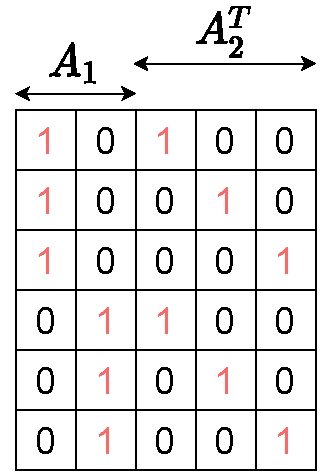
\includegraphics[height=0.25\textheight,keepaspectratio]{./Chapitre2/fig/matrix.pdf}
  \caption{An example of the matrix $A_{12}$ when $n_1=2$ and $n_2=3$.}
  \label{fig:matrix_a12}
\end{figure}

We also have that, the condition $P = P_1 \otimes P_2$ can be rewritten as
$\text{mat}(P) = \vect(P_1) \vect(P_2)^T$. By Lemma 2.1 in \citep{Joel93}, $\text{rank}_+(A) = 1$
if and only if there exist two non-negative vectors $u,v$ such that
$A = u v^T$. Thus, the factorization constraint is equivalent to
$\text{rank}_+\big( \text{mat}(P) \big) = 1$.

Now, denote $L= \text{mat}(C)$ and $M = n_1 n_2, N = n_3 n_4$. COOT can be rewritten as
\begin{equation*}
  \begin{split}
    \min_{Q \in \bbR^{M \times N}_{\geq 0}} &\langle L, Q \rangle \\
    \text{ such that } & A_{12}^T Q 1_N = \mu_{12} \\
    &A_{34}^T Q^T 1_M = \mu_{34} \\
    &\text{rank}_{+}(Q) = 1,
  \end{split}
\end{equation*}
which is a variation of the non-negative rank-$1$ OT problem.

%%%%%%%%%%%%%%%%%%%%%%%%%%%%%%%%%%%%%%
\subsection{Co-Optimal Transport as factored multi-marginal OT} \label{subsec:MMOT_DC}

Note that we can rewrite COOT as a variation of multi-marginal OT (MMOT) problem.
To see this, first, we recall some related concepts.
Given an integer $N \geq 1$, for any positive integers $a_1,..., a_N$, we call
$P \in \bbR^{a_1 \times ... \times a_N}$ a $N$-D tensor. In particular,
a $1$-D tensor is a vector and $2$-D tensor is a matrix.
A tensor is a probability tensor if its entries are non-negative and the sum of all entries is $1$.
Given $N$ probability vectors $\mu_1, ..., \mu_N$, we write $\mu = (\mu_n)_{n=1}^N$.
We denote $\Sigma$ the set of $N$-D probability tensors and $U(\mu) \subset \Sigma$ the set of non-negative tensors whose $N$
marginal distributions are $\mu_1, ..., \mu_N$. In this case, any coupling in $U(\mu)$ is said to be \textit{admissible}.

Given a collection of $N$ histograms $\mu = (\mu_n \in \bbR^{a_n})_{n=1}^N$
and a $N$-D cost tensor $C \in \bbR^{a_1 \times ... \times a_N}$, the MMOT problem reads
\begin{equation*}
  \text{MMOT}(\mu) = \inf_{P \in U(\mu)} \langle C, P \rangle.
\end{equation*}
In practice, such a formulation is intractable to optimize in a discrete setting as it results in a linear program where the number
of constraints grows exponentially in $N$. A more tractable strategy for solving MMOT is to consider the following entropic
regularization problem
\begin{equation} \label{MMOT_primal}
  \inf_{P \in U(\mu)} \langle C, P \rangle + \varepsilon H(P).
\end{equation}
which can be solved using Sinkhorn's algorithm \citep{Benamou14}. We refer the interested reader to Supplementary materials for algorithmic details.

\paragraph{Derivation of the Sinkhorn algorithm in entropic MMOT.} The corresponding entropic dual problem of the primal problem
\ref{MMOT_primal} reads
\begin{equation*}
  \sup_{f_n \in \bbR^{a_n}} \sum_{n=1}^N \langle f_n, \mu_n \rangle -
  \varepsilon \sum_{i_1,...,i_N} \exp\Big( \frac{\sum_n (f_n)_{i_n} - C_{i_1,...,i_N}}{\varepsilon} \Big) + \varepsilon.
\end{equation*}
For each $n \in [N]$ and $i_n \in [a_n]$, the first order optimality condition reads
\begin{equation*}
  0 = (\mu_n)_{i_n} - \exp\big( \frac{(f_n)_{i_n}}{\varepsilon} \big)
  \sum_{i_{-n}} \exp\Big( \frac{\sum_{j \neq n} (f_j)_{i_j} - C_{i_1,...,i_N}}{\varepsilon} \Big),
\end{equation*}
where, with some abuse of notation, we write $i_{-n} = (i_1, ..., i_{n-1}, i_{n+1}, ..., i_N)$. Or, equivalently
\begin{equation*}
  (f_n)_{i_n} = \varepsilon \log (\mu_n)_{i_n} - \varepsilon \log \sum_{i_{-n}}
  \exp\Big( \frac{\sum_{j \neq n} (f_j)_{i_j} - C_{i_1,...,i_N}}{\varepsilon} \Big),
\end{equation*}
or even more compact form
\begin{equation*}
  f_n = \varepsilon \log \mu_n - \varepsilon \log \sum_{i_{-n}}
  \exp\Big( \frac{\sum_{j \neq n} (f_j)_{i_j} - C_{\cdot, i_{-n}}}{\varepsilon} \Big).
\end{equation*}
Using the primal-dual relation, we obtain the minimiser of the primal problem \ref{MMOT_primal} by
\begin{equation*}
  P_{i_1,...,i_N} = \exp\Big( \frac{\sum_n (f_n)_{i_n} - C_{i_1,...,i_N}}{\varepsilon} \Big),
\end{equation*}
for $i_n \in [a_n]$, with $n \in [N]$.
%%%%%%%%%%%%%%%%%%%%%%%%%%%%%%%%%%%%%%%%%
Similar to the entropic OT, the Sinkhorn algorithm \ref{algo:dual_mmot} is also usually implemented in log-domain to avoid numerical instability.
\begin{algorithm}[h]
  \caption{Sinkhorn algorithm for the entropic MMOT problem \ref{MMOT_primal} from \citep{Benamou14}.}
  \textbf{Input.} Histograms $\mu_1,...,\mu_N$, hyperparameter $\varepsilon > 0$, cost tensor $C$ and
  tuple of initial dual vectors $(f^{(0)}_1, ... f^{(0)}_N)$.

  \textbf{Output.} Optimal transport plan $P$ and tuple of dual vectors $(f_1, ... f_N)$ (optional).
  \begin{enumerate}
    \item While not converge: for $n = 1, ..., N$,
    \begin{equation*}
      \begin{split}
        f^{(t+1)}_n &= \varepsilon \log \mu_n - \varepsilon \log \sum_{i_{-n}}
        \Big[ \exp\Big( \frac{\sum_{j < n} (f^{(t+1)}_j)_{i_j} + \sum_{j > n} (f^{(t)}_j)_{i_j} -
        C_{\cdot, i_{-n}}}{\varepsilon} \Big) \Big].
      \end{split}
    \end{equation*}
    \item Return tensor $P$, where for $i_n \in [a_n]$, with $n \in [N]$,
    \begin{equation*}
      P_{i_1,...,i_N} = \exp\Big( \frac{\sum_n (f_n)_{i_n} - C_{i_1,...,i_N}}{\varepsilon} \Big).
    \end{equation*}
  \end{enumerate}
  \label{algo:dual_mmot}
\end{algorithm}

Now, it is easy to see that COOT can be rewritten as
\begin{align*}
  \inf_{\gamma \in U_2} \langle C, \gamma \rangle
\end{align*}
where $U_2 = {\gamma \in U(\mu): \gamma = \pi^s }$

\paragraph{Contributions} We define and study a general MMOT problem with structural penalization on the coupling matrix.
We start by showing that a such formulation includes several popular OT methods as special cases and allows to gain deeper insights
into them. We further consider a relaxed problem where the hard constraint is replaced by a regularization term and show that it leads
to an instance of the difference of convex programming problem. A numerical study of the solutions obtained when solving the latter
in cases of interest highlights their competitive performance when compared to solutions provided by the optimization
strategies used previously.

\subsubsection*{Factored MMOT and its relaxation}
We start by giving several definitions used in the following parts of the paper.
%We call $P \in \bbR^{a_1 \times ... \times a_N}$ a $N$-D tensor. When $N=1$, we simply call it a vector and when $N=2$,
%it is a matrix.
\begin{definition}[Tuple partition]
 Given two integers $N \geq M \geq 2$, a sequence of tuples $\mathcal T = (\mathcal T_m)_{m=1}^M$, is called a
 \underline{tuple partition} of the $N$-tuple $(1,...,N)$ if the tuples $\mathcal T_1, ..., \mathcal T_M$ are nonempty and disjoint,
 and their concatenation in this order gives $(1,...,N)$.
\end{definition}
Here, we implicitly take into account the order of the tuple, which is not the case for the partition of the set $[N]$. If
there exists a tuple in $\mathcal T$ which contains only one element, then we say $\mathcal T$ is \textit{degenerate}.

\begin{definition}[Marginal tensor]
  Given a tensor $P \in \bbR^{a_1 \times ... \times a_N}$ and a tuple partition $\mathcal T = (\mathcal T_m)_{m=1}^M$,
  we call $P_{\# \mathcal T_m}$ its \underline{$\mathcal T_m$-marginal tensor}, by summing $P$ over all dimensions not in $\mathcal T_m$.
  We write $P_{\# \mathcal T} = P_{\# \mathcal T_1} \otimes ... \otimes P_{\# \mathcal T_M} \in \bbR^{a_1 \times ... \times a_N}$
  the tensor product of its marginal tensors.
\end{definition}
For example, for $M=N=2$, we have $\mathcal T_1 = (1)$ and $\mathcal T_2 = (2)$. So, given a matrix
$P \in \bbR^{a_1 \times a_2}$, its marginal tensors $P_{\# \mathcal T_1}$ and $P_{\# \mathcal T_2}$ are simply vectors in
$\bbR^{a_1}$ and $\bbR^{a_2}$, respectively, defined by $(P_{\# \mathcal T_1})_i = \sum_j P_{ij}$ and
$(P_{\# \mathcal T_2})_j = \sum_i P_{ij}$ for $(i,j) \in [a_1] \times [a_2]$. The tensor product
$P_{\# \mathcal T} \in \bbR^{a_1 \times a_2}$ is then defined by
$(P_{\#\mathcal T})_{ij} = (P_{\# \mathcal T_1})_i (P_{\# \mathcal T_2})_j$.

Clearly, if $P$ is a probability tensor, then so are its marginal tensors and tensor product.

Suppose $\mathcal T_m = (p,...,q)$ for some $m \in [M]$ and $1 \leq p \leq q \leq N$. We denote
$\Sigma_{\mathcal T_m}$ the set of probability tensors in $\bbR^{a_p \times ... \times a_q}$ and
$U_{\mathcal T_m} \subset \Sigma_{\mathcal T_m}$ the set
of probability tensors in $\bbR^{a_p \times ... \times a_q}$ whose $(r)$-marginal vector is $\mu_r$, for every $r = p,...,q$.

%%%%%%%%%%%%%%%%%%%%%%%%%%%%%%%
\begin{definition}[Factored MMOT]
  Given a collection of histograms $\mu = (\mu_n)_{n=1}^N$ and a tuple partition $\mathcal T = (\mathcal T_m)_{m=1}^M$,
  we consider the following OT problem
  \begin{equation} \label{factor_mmot}
    \text{F-MMOT}( \mathcal T, \mu) = \inf_{P \in U_{\mathcal T}} \langle C, P \rangle,
  \end{equation}
  where $U_{\mathcal T} \subset U(\mu)$ is the set of admissible couplings which can be factorized as a tensor product of $M$
  component probability tensors in $\Sigma_{\mathcal T_1}, ..., \Sigma_{\mathcal T_M}$.
\end{definition}
Several remarks are in order here. First, one should note that the partition considered above is in general not degenerate meaning
that the decomposition can involve tensors of an arbitrary order $<N$. Second, the decomposition in this setting depicts the prior
knowledge regarding the tuples of measures which should be independent: the couplings for the measures from different tuples will
be degenerate and the optimal coupling tensor will be reconstructed from couplings of each tuple separately.
Third, suppose the partition $(\mathcal T_m)_{m=1}^M$ is not degenerate and $M=2$, i.e. the tensor is factorized as product of
two tensors, the problem \cref{factor_mmot} is equivalent to a variation of low non-negative rank OT problem (see Appendix for a proof).

As for the existence of the solution to this problem, we have that $U_{\mathcal T}$ is compact because it is a close subset of the
compact set $U(\mu)$, which implies that the problem \cref{factor_mmot} always admits a solution. Furthermore, observe that
\begin{equation*}
  \begin{split}
    U_{\mathcal T} &= \{ P \in U(\mu): P = P_1 \otimes ... \otimes P_M, \text{where } P_m \in \Sigma_{\mathcal T_m}, \forall m = 1,...,M \} \\
    &= \{ P \in \Sigma: P = P_1 \otimes ... \otimes P_M, \text{where } P_m \in U_{\mathcal T_m}, \forall m = 1,...,M \}.
  \end{split}
\end{equation*}
Thus, the problem F-MMOT can be rewritten as
\begin{equation*}
  \text{F-MMOT}( \mathcal T, \mu) = \inf_{\substack{P_m \in U_{\mathcal T_m} \\ \forall m = 1,...,M}}
  \langle C, P_1 \otimes ... \otimes P_M \rangle.
\end{equation*}
So, if $\mathcal T_1,...,\mathcal T_M$ are $2$-tuples and two marginal distributions corresponding to each $U_{\mathcal T_m}$ are
identical and uniform, then by Birkhoff's theorem \citep{Birkhoff46}, the problem \ref{factor_mmot} admits an optimal solution in
which each component tensor $P_m$ is a permutation matrix.

\paragraph{Two special cases.} When $N = 4$ and $M=2$ with $\mathcal T_1 = (1,2)$ and $\mathcal T_2 = (3,4)$, the problem
\ref{factor_mmot} becomes the CO-Optimal transport (COOT), where the two component tensors are known as
\textit{sample} and \textit{feature} couplings. If furthermore, $a_1 = a_3, a_2=a_4$, and $\mu_1 = \mu_3, \mu_2=\mu_4$, it becomes a
lower bound of the discrete Gromov-Wasserstein (GW) distance \citep{Memoli11}. This means that our formulation can be seen as a
generalization of several OT formulations.

%%%%%%%%%%%%%%%%%%%%%%%%%%%%%%%%%%%%%%%%%%%%%
Observe that if a probability tensor $P$ can be factorized as a tensor product of probability tensors, i.e.
$P = P_1 \otimes ... \otimes P_M$, then each $P_m$ is also the $\mathcal T_m$-marginal tensor of $P$. In this case,
we have $P = P_{\# \mathcal T}$. This prompts us to consider the following relaxation of factored MMOT, where the hard constraint
$U_{\mathcal T}$ is replaced by a regularization term.
\begin{definition}[Relaxed Factored MMOT]
  Given $\varepsilon \geq 0$, a collection of measures $\mu$ and a tuple partition $\mathcal T$,
  we define the following problem:
  \begin{equation} \label{relax_mmot}
    \text{MMOT-DC}_{\varepsilon}( \mathcal T, \mu) =
    \inf_{P \in U(\mu)} \langle C, P \rangle + \varepsilon \kl(P \vert P_{\# \mathcal T}).
  \end{equation}
\end{definition}
From the exposition above, one can guess that this relaxation is reminiscent of the entropic regularization in MMOT and
coincides with it when $M = N$. As such, it also recovers the classical entropic OT. One should note that the choice of the KL
divergence is not arbitrary and its advantage will become clear when it comes to the algorithm. %A well known
A special case of the problem \ref{relax_mmot} is when $M = N$, we recover the entropic-regularized MMOT problem, up to a constant.

After having defined the two optimization problems, we now set on exploring their theoretical properties.

\subsubsection*{Theoretical properties}
%The following properties are direct consequences of the definition.
Intuitively, the relaxed problem is expected to allow for solutions with a lower value of the final objective function. We formally prove the validity of this intuition below.
%%%%%%%%%%%%%%%%%%%%%%%%%%%%%%%%%%%%%%%%%%%%%
\begin{proposition}[Preliminary properties]
  \label{MMOT_dc_prop}
  Given a collection of histograms $\mu$ and a tuple partition $\mathcal T$,
  \begin{enumerate}
    \item For every $\varepsilon \geq 0$, we have $\text{MMOT}(\mu) \leq
    \text{MMOT-DC}_{\varepsilon}(\mathcal T, \mu) \leq \text{F-MMOT}( \mathcal T, \mu)$.
    \item For every $\varepsilon > 0, \text{MMOT-DC}_{\varepsilon}( \mathcal T, \mu ) = 0$ if and only if
    $\text{F-MMOT} (\mathcal T, \mu) = 0$.
  \end{enumerate}
\end{proposition}
%%%%%%%%%%%%%%%%%%%%%%%%%%%%%%%%%%%%%%%%%%%%%
An interesting property of MMOT-DC is that it interpolates between MMOT and F-MMOT. Informally,
for very large $\varepsilon$, the KL divergence term dominates, so the optimal transport plans tend to be factorizable.
On the other hand, for very small $\varepsilon$, the KL divergence term becomes negligible and we approach MMOT.
The result below formalizes this intuition.
%%%%%%%%%%%%%%%%%%%%%%%%%%%%%%%%%%%%%%%%%%%%%
\begin{proposition}[Interpolation between MMOT and F-MMOT]
  \label{interpolation_prop}
  For any tuple partition $\mathcal T$ and for $\varepsilon > 0$,
  let $P_{\varepsilon}$ be a minimiser of the problem $\text{MMOT-DC}_{\varepsilon}(\mathcal T, \mu)$.
  \begin{enumerate}
    \item When $\varepsilon \to \infty$, one has $\text{MMOT-DC}_{\varepsilon}(\mathcal T, \mu) \to
    \text{F-MMOT}(\mathcal T, \mu)$. In this case, any cluster point of the sequence of minimisers
    $(P_{\varepsilon})_{\varepsilon}$ is a minimiser of $\text{F-MMOT}(\mathcal T, \mu)$.

    \item When $\varepsilon \to 0$, then $\text{MMOT-DC}_{\varepsilon}(\mathcal T, \mu) \to \text{MMOT}(\mu)$.
    In this case, any cluster point of the sequence of minimisers $(P_{\varepsilon})_{\varepsilon}$ is a minimiser of
    $\text{MMOT}(\mu)$.
  \end{enumerate}
\end{proposition}
%%%%%%%%%%%%%%%%%%%%%%%%%%%%%%%%%%%%%%%%%%%%%
\paragraph{GW distance revisited.} Somewhat surprisingly, the relaxation \ref{relax_mmot} also allows us to prove the equality
between GW distance and COOT in the discrete setting. Let $\mathcal X$ be a
finite subset (of size $m$) of a certain metric space. Denote $C_x \in \bbR^{m \times m}$ its similarity matrix (e.g. distance
matrix). We define similarly the set $\mathcal Y$ of size $n$ and the corresponding similarity matrix $C_y \in \bbR^{n \times n}$.
We also assign two discrete probability measures $\mu_x \in \bbR^m$ and $\mu_y \in \bbR^n$ to $\mathcal X$ and $\mathcal Y$,
respectively. The GW distance is then defined as
\begin{equation*}
  \gw(C_x, C_y) = \inf_{Q \in U(\mu_x, \mu_y)} \langle L(C_x, C_y), Q \otimes Q \rangle,
\end{equation*}
and the COOT reads
\begin{equation*}
  \coot(C_x, C_y) = \inf_{\substack{Q_s \in U(\mu_x, \mu_y) \\ Q_f \in U(\mu_x, \mu_y)}}
  \langle L(C_x, C_y), Q_s \otimes Q_f \rangle,
\end{equation*}
where $L(C_x,C_y) \in \bbR^{m \times n \times m \times n}$ represents the $4$-D cost tensor induced by the matrices $C_x$ and $C_y$,
and $U(\mu, \nu)$ is the set of couplings in $\bbR^{m \times n}_{\geq 0}$ whose two marginal distributions are $\mu$ and
$\nu$. When $C_x$ and $C_y$ are two squared Euclidean distance matrices, and $L(C_x,C_y)$ is of the form
$\big(L(C_x,C_y)\big)_{i,j,k,l} = \vert (C_x)_{i,k} - (C_y)_{j,l} \vert^2$, it can be shown that the GW distance is equal
to the COOT. This is also true when $L(C_x, C_y)$ is a negative definite kernel \citep{Sejourne20}.
Here, we establish a weaker case where this equality still holds.
%%%%%%%%%%%%%%%%%%%%%%%%%%%%%%%%%%%%%%%%%%%%%
\begin{corollary} \label{kernel_gw_coot}
  If $L(C_x, C_y)$ defines a conditionally negative definite kernel on $(\mathcal X \times \mathcal Y)^2$, then we have the equality
  between GW distance and COOT. Furthermore, if $(Q_s^*,Q_f^*)$ is a solution of the COOT problem, then $Q_s^*$ and $Q_f^*$ are
  two solutions of the GW problem. In particular, when $L(C_x, C_y)$ induces a strictly positive definite kernel
  $\exp \big( -\frac{L(C_x, C_y)}{\varepsilon} \big)$, for every $\varepsilon > 0$, we have $Q_s^* = Q_f^*$.
\end{corollary}
%%%%%%%%%%%%%%%%%%%%%%%%%%%%%%%%%%%%%%%%%%%%%
The proof relies on the connection between MMOT-DC and COOT shown in the \cref{interpolation_prop},
and given a
$4$-D solution of MMOT-DC, we can construct another $4$-D solutions whose
$\mathcal T_1$ and $\mathcal T_2$-marginal matrices are identical,
under the assumption of the cost tensor. The proof of the second claim is deferred to the Appendix.
Note that, this result is more general than the one in the previous section, where

\subsubsection*{Numerical solution} \label{sec:algo}
%%%%%%%%%%%%%%%%%%%%%%%%%%%%%%%%%%%%%%%%%%%%%
We now turn to the computational aspect of the problem \ref{relax_mmot}. First, note that for any tuple partition
$\mathcal T = (\mathcal T_m)_{m=1}^M$ and probability tensor $P$, the KL divergence term can be decomposed as
\begin{equation*}
  \kl(P \vert P_{\# \mathcal T}) = H(P) - \sum_{m=1}^m H_m(P),
\end{equation*}
where the function $H_m$ defined by $H_m(P) := H(P_{\# \mathcal T_m})$ is continuous and convex with respect to $P$.
Now, the problem \ref{relax_mmot} becomes
\begin{equation} \label{relax}
  \text{MMOT-DC}_{\varepsilon}(\mathcal T, \mu) = \inf_{P \in U(\mu)}
  \langle C, P \rangle + \varepsilon H(P) - \varepsilon \sum_{m=1}^M H_m(P).
\end{equation}
This is nothing but a Difference of Convex (DC) programming problem (which explains the name MMOT-DC),
thanks to the convexity of the set $U(\mu)$ and the entropy function $H$. Thus, it can be solved
by the classic DC algorithm
\footnote{The DC algorithm is very closely related to Convex-concave procedure, majorization-minimization algorithm, Successive Linear
Approximation. For a detailed discussion on the subtle distinction amongst these name, see
\citep{}} \citep{Tao86,Tao97} as follows: at the iteration $t$,
\begin{enumerate}
  \item Calculate $G^{(t)} \in \partial(\sum_{m=1}^M H_m)(P^{(t)})$.
  \item Solve $P^{(t+1)} \in \arg\min_{P \in U(\mu)} \langle C -
  \varepsilon G^{(t)}, P \rangle + \varepsilon H(P)$.
\end{enumerate}
%%%%%%%%%%%%%%%%%%%%%%%%%%%%%%%%%%%%%%%%%%%%%%
This algorithm is very easy to implement. Indeed, the second step is an entropic-regularized MMOT problem, which admits a unique
solution, thanks to the strict convexity of the objective function. Such solution can be found by the Sinkhorn algorithm
\ref{algo:dual_mmot}. In the first step, the gradient can be calculated explicitly.
For the sake of simplicity, we illustrate the calculation in a simple case, where $M=2$ and $N=4$ with
$\mathcal T_1$ and $\mathcal T_2$ are two $2$-tuples. The function $H_1 + H_2$ is continuous, so
$G^{(t)} = \nabla_P (H_1 + H_2)(P^{(t)})$. Given a $4$-D probability tensor $P$, we have
\begin{equation*}
  H_1(P) + H_2(P) = \sum_{i,j,k,l} P_{i,j,k,l}
  \log\big( \sum_{i,j} P_{i,j,k,l} \big) + P_{i,j,k,l} \log\big( \sum_{k,l} P_{i,j,k,l} \big).
\end{equation*}
So,
\begin{equation*} \label{optim_condition}
  \frac{\partial (H_1 + H_2)}{\partial P_{i,j,k,l}} = \log \left( \sum_{i,j} P_{i,j,k,l} \right) +
  \frac{P_{i,j,k,l}}{\sum_{i,j} P_{i,j,k,l}} +
  \log \left( \sum_{k,l} P_{i,j,k,l} \right) + \frac{P_{i,j,k,l}}{\sum_{k,l} P_{i,j,k,l}}.
\end{equation*}
The complete DC algorithm for the problem \ref{relax} can be found in the algorithm \ref{algo:dc_MMOT}.
%%%%%%%%%%%%%%%%%%%%%%%%%%%%%%%%%%%%%%%%%%%%%%
\begin{algorithm}[h]
  \caption{DC algorithm for the problem \ref{relax_mmot}.}
  \textbf{Input.} Cost tensor $C$, tuple partition $(\mathcal T_m)_{m=1}^M$, collection of histograms $\mu = (\mu_n)_{n=1}^N$,
  hyperparameter $\varepsilon > 0$, initialization $P^{(0)}$, tuple of initial dual vectors for the
  Sinkhorn step $(f_1^{(0)},...,f_N^{(0)})$.

  \textbf{Output.} Tensor $P \in U(\mu)$.

  While not converge
  \begin{enumerate}
    \item Gradient step: compute the gradient of the convex term $G^{(t)} = \sum\limits_{m=1}^M \nabla_P H_m(P^{(t)})$.
    \item Sinkhorn step: solve
    \begin{equation*}
      P^{(t+1)} = \arg\min_{P \in U(\mu)} \langle C - \varepsilon G^{(t)}, P \rangle + \varepsilon H(P),
    \end{equation*}
    using the Sinkhorn algorithm \ref{algo:dual_mmot}, with the tuple of initial dual vectors $(f_1^{(0)},...,f_N^{(0)})$.
  \end{enumerate}
  \label{algo:dc_MMOT}
\end{algorithm}
%%%%%%%%%%%%%%%%%%%%%%%%%%%%%%%%%%%%%%%%%%%%%
We observed that initialization is crucial to the convergence of algorithm, which
is not surprising for a non-convex problem. To accelerate the algorithm for large $\varepsilon$,
we propose to use the warm-start strategy, which is similar to the one used in the entropic OT problem with very
small regularization parameter \citep{Schmitzer19}. Its idea is simple: we consider an increasing finite sequence
$(\varepsilon_n)_{n=0}^N$ approaching $\varepsilon$ such that the solution $P_{\varepsilon_0}$ of the problem
$\text{MMOT-DC}_{\varepsilon_0}(\mathcal T, \mu)$ can be estimated quickly and accurately using the initialization $P^{(0)}$. Then we solve each
successive problem $\text{MMOT-DC}_{\varepsilon_n}(\mathcal T, \mu)$ using the previous solution $P_{\varepsilon_{n-1}}$ as initialization. Finally,
the problem $\text{MMOT-DC}_{\varepsilon}(\mathcal T, \mu)$ is solved using the solution $P_{\varepsilon_N}$ as initialization.

%%%%%%%%%%%%%%%%%%%%%%%%%%%%%%%%%%%%%%%%%%%%%%
\subsubsection{Experimental evaluation} \label{sec:exp}
%%%%%%%%%%%%%%%%%%%%%%%%%%%%%%%%%%%%%%%%%%%%%%
In this section, we illustrate the use of MMOT-DC on simulated data. Rather than performing experiments in full generality,
we choose the setting where $N = 4$ and $M=2$ with $\mathcal T_1 = (1,2)$ and $\mathcal T_2 = (3,4)$,
so that we can compare MMOT-DC with other popular solvers of COOT and GW distance. Given two matrices $X$ and $Y$, we always consider the $4$-D cost tensor $C$,
where $C_{i,j,k,l} = \vert X_{i,k} - Y_{j,l} \vert^2$. On the other hand, we are not interested in the $4$-D minimiser of MMOT-DC,
but only in its two $\mathcal T_1, \mathcal T_2$-marginal matrices.

\paragraph{Solving COOT on a toy example.} We generate a random matrix $X \in \bbR^{30 \times 25}$, whose entries are drawn independently
from the uniform distribution on the interval $[0,1)$. We equip the rows and columns of $X$ with two discrete uniform distributions
on $[30]$ and $[25]$. We fix two permutation matrices $Q_s \in \bbR^{30 \times 30}$ (called sample permutation) and
$Q_f \in \bbR^{25 \times 25}$ (called feature permutation), then calculate $Y = Q_s X Q_f$. We also equip the rows and columns of $Y$
with two discrete uniform distributions on $[30]$ and $[25]$.

It is not difficult to see that $\coot(X,Y) = 0$ because $(Q_s, Q_f)$ is a solution. As COOT is a special case of F-MMOT,
we see that $\text{MMOT-DC}_{\varepsilon}(\mathcal T, \mu) = 0$, for every $\varepsilon > 0$,
by proposition \ref{MMOT_dc_prop}. In this experiment, we will check if marginalizing the minimizer of MMOT-DC allows us to recover
the permutation matrices $Q_s$ and $Q_f$.
As can be seen from the figure \ref{fig:permu}, MMOT-DC can recover the permutation positions, for various
values of $\varepsilon$. On the other hand, it can not recover the true sparse permutation matrices because the Sinkhorn algorithm
applied to the MMOT problem implicitly results in a dense tensor, thus having dense marginal matrices. For this reason,
the loss only remains very close to zero, but never exactly.
%%%%%%%%%%%%%%%%%%%%%%%%%%%%%%%%%%%%%%%
\begin{figure}[t]
  \centering
  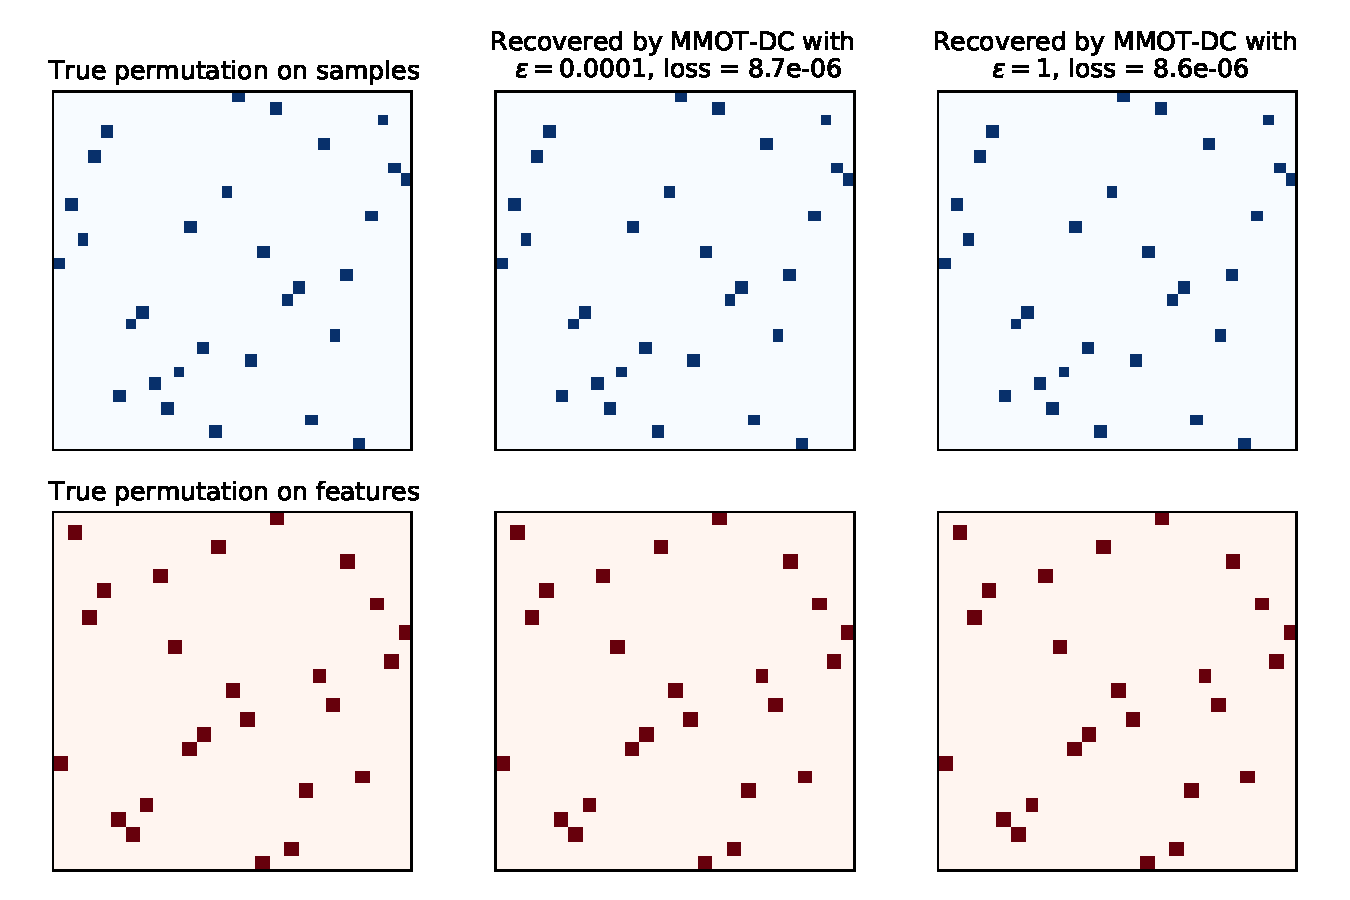
\includegraphics[width=0.8\textwidth,height=0.8\textheight,keepaspectratio]{./Chapitre2/fig/compare_methods.pdf}
  \caption{Couplings generated by COOT and MMOT-DC on the matrix recovering task.}
  \label{fig:permu}
\end{figure}
%%%%%%%%%%%%%%%%%%%%%%%%%%%%%%%%%%%%%%%
We also plot, with some abuse of notation, the histograms of the difference between
the $(1,3), (1,4), (2,3), (2,4)$-marginal matrices of MMOT-DC and their corresponding counterparts from F-MMOT.
In this example, in theory, as the optimal tensor $P$ of F-MMOT can be factorized as
$P = P_{\# \mathcal T_1} \otimes P_{\# \mathcal T_2} = Q_s \otimes Q_f$,
it is immediate to see that $P_{\# (1,3)} = P_{\# (1,4)} = P_{\# (2,3)} = P_{\# (2,4)} \in \bbR^{30 \times 25}$
are uniform matrices whose entries are $\frac{1}{750}$.
%%%%%%%%%%%%%%%%%%%%%%%%%%%%%%%%%%%%%%%
\begin{figure}[t]
  \centering
  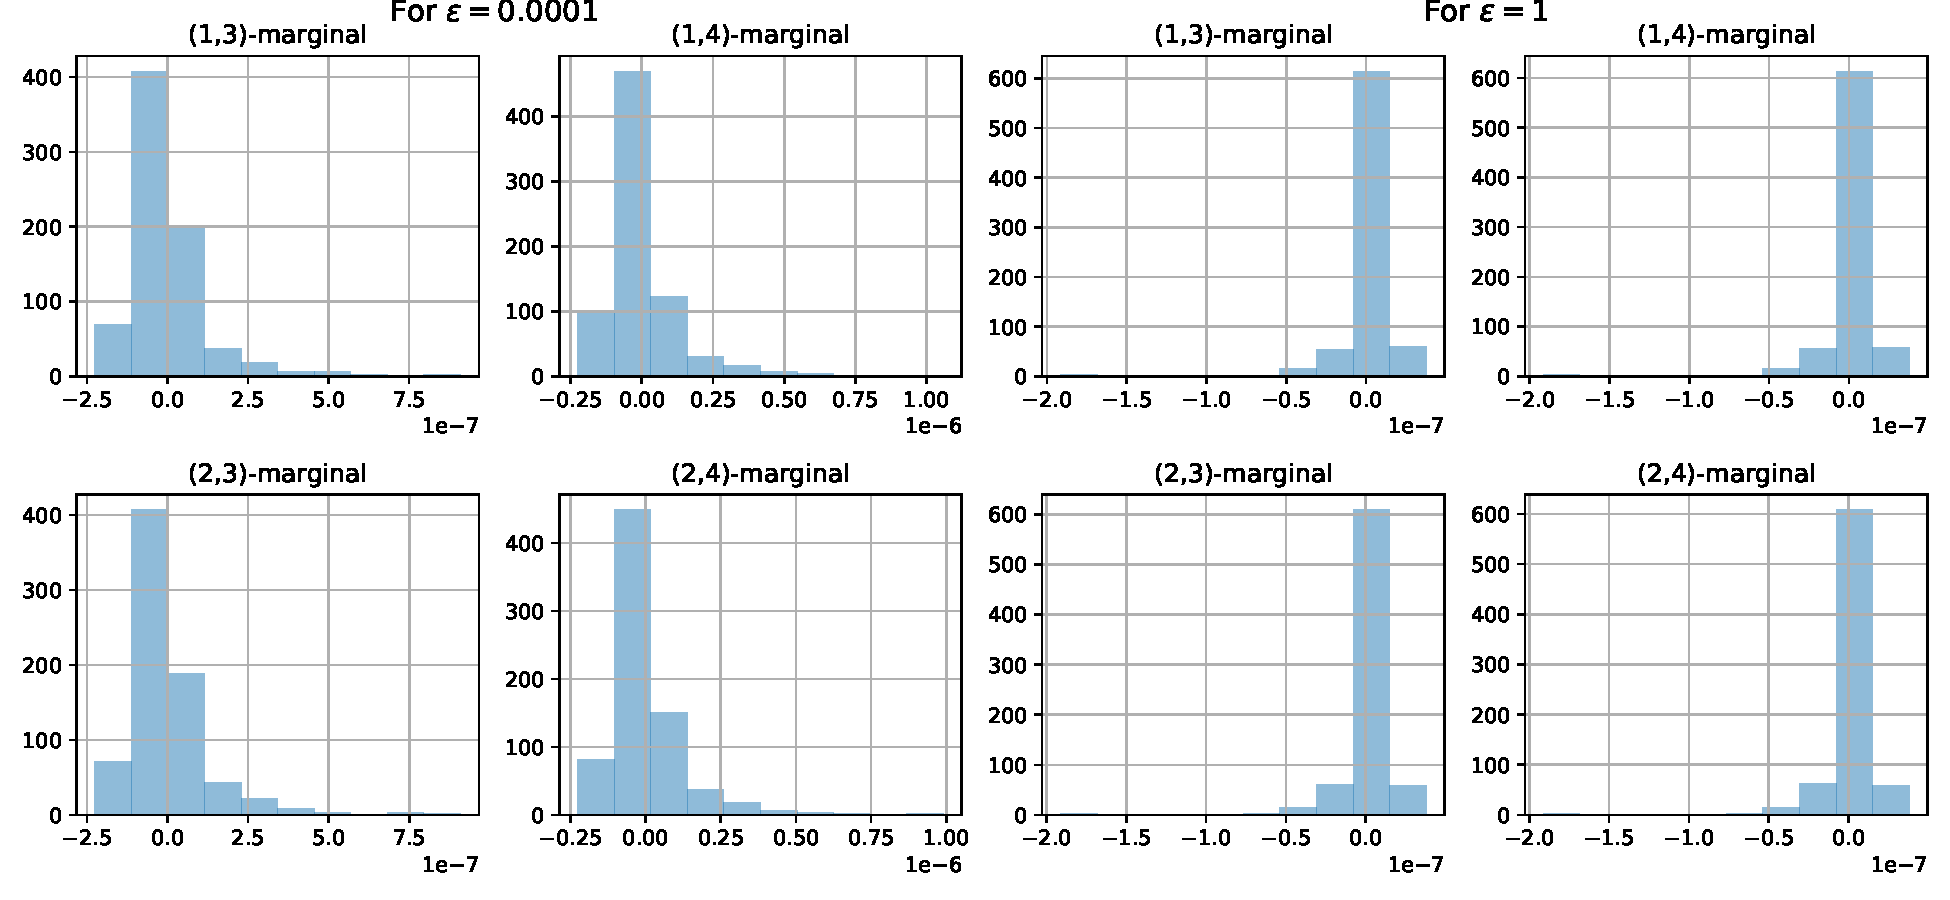
\includegraphics[width=1.\textwidth,height=1.\textheight,keepaspectratio]{./Chapitre2/fig/other_marginals.pdf}
  \caption{Histograms of difference between true independent marginal matrices and their approximations. We see that the marginal matrices obtained
  by the algorithm \ref{algo:dc_MMOT} approximate well the theoretical uniform matrices.}
  \label{fig:other_marg}
\end{figure}

%%%%%%%%%%%%%%%%%%%%%%%%%%%%%%%%%%%%%%%
\paragraph{Quality of the MMOT-DC solutions. \label{expe:2}}

% In the following example, our evaluation metric is the COOT loss $\langle C, P \otimes Q \rangle$,
% where the smaller the loss, the better.

Now, we consider the situation where the true matching between two matrices is not known in advance and investigate the quality
of the solutions returned by MMOT-DC to solve the COOT and GW problems. This means that we will look at the COOT loss
$\langle C, Q_s \otimes Q_f \rangle$, where the smaller the loss, the better when using both exact COOT and GW solvers
and our relaxation.

We generate two random matrices $X \in \bbR^{20 \times 3}$ and $Y \in \bbR^{30 \times 2}$,
whose entries are drawn independently from the uniform distribution on the interval $[0,1)$. Then we calculate two corresponding
squared Euclidean distance matrices of size $20$ and $30$. Their rows and columns are equipped with the discrete
uniform distributions. In this case, \citep{Redko20} show that the COOT loss coincides with the GW distance, and the
Block Coordinate Descent (BCD) algorithm used to approximate COOT is equivalent to the Frank-Wolfe algorithm \citep{Frank56}
used to solve the GW distance.

We compare four solvers:
\begin{enumerate}
  \item The Frank-Wolfe algorithm to solve the GW distance (GW-FW).

  \item The projected gradient algorithm to solve the entropic GW distance \citep{Peyre16} (EGW-PGD). We choose the regularization
  parameter from $\{0.0008, 0.0016, 0.0032, 0.0064, 0.0128, 0.0256 \}$ and pick the one which corresponds to smallest COOT loss.

  \item The Block Coordinate Descent algorithm to approximate the entropic COOT \citep{Redko20}
  (EGW-BCD), where two additional KL divergences corresponding to two couplings are introduced.
  Both regularization parameters are tuned from $\{0, 0.0005, 0.001, 0.005, 0.01, 0.05, 0.1, 0.5, 1 \}$,
  where $0$ means that there is no regularization term for the corresponding coupling and we pick the pair whose COOT loss is the smallest.

  \item The algorithm \ref{algo:dc_MMOT} to solve the MMOT-DC. We tune
  $\varepsilon \in \{1, 1.4, 1.8, 2.2, 2.6\}$ and we pick the one which corresponds to smallest COOT loss.
\end{enumerate}
For GW-FW and EGW-PGD, we use the implementation from the library \texttt{PythonOT} \citep{Flamary21}.

Given two random matrices, we record the COOT loss corresponding to the solution generated by each method.
We simulate this process $70$ times and compare their overall performance. We can see in Table \ref{tab:gw} the average value and
standard deviation and the comparison for the values of the loss between the different algorithms in Figure \ref{fig:gw}.
The performance is quite similar across methods with a  slight advantage for EGW-PGD. This is in itself a very
interesting result that has never been noted, to the best of our knowledge: the reason that the entropic version of GW can
provide better solution than solving the exact problem, may be due to the "convexification" of the problem, thanks to the entropic
regularization. Our approach is also interestingly better than the exact GW-FW, which illustrates that the relaxation might help in
finding better solutions despite the non-convexity of the problem.
%%%%%%%%%%%%%%%%%%%%%%%%%%%%%%%%%%%%%%%
\begin{table}[t]
  % \vskip 0.15in
  \begin{center}
    \begin{small}
      \begin{sc}
        \begin{tabular}{|c|c|c|c|}
          \hline
          GW-FW & EGW-PGD & EGW-BCD & MMOT-DC \\
          \hline
          0.0829 ($\pm$ 0.0354) & \textbf{0.0786 ($\pm$ 0.0347)} & 0.0804 ($\pm$ 0.0353) & 0.0822 ($\pm$ 0.0364) \\
          \hline
        \end{tabular}
      \end{sc}
    \end{small}
  \end{center}
  \caption{Average and standard deviation of COOT loss of the solvers. MMOT-DC is competitive to other solvers,
  except for EGW-PGD and EGW-BCD.
  \label{tab:gw}}
  % \vskip -0.1in
\end{table}

%%%%%%%%%%%%%%%%%%%%%%%%%%%%%%%%%%%%%%%
\begin{figure}[t]
	\centering
	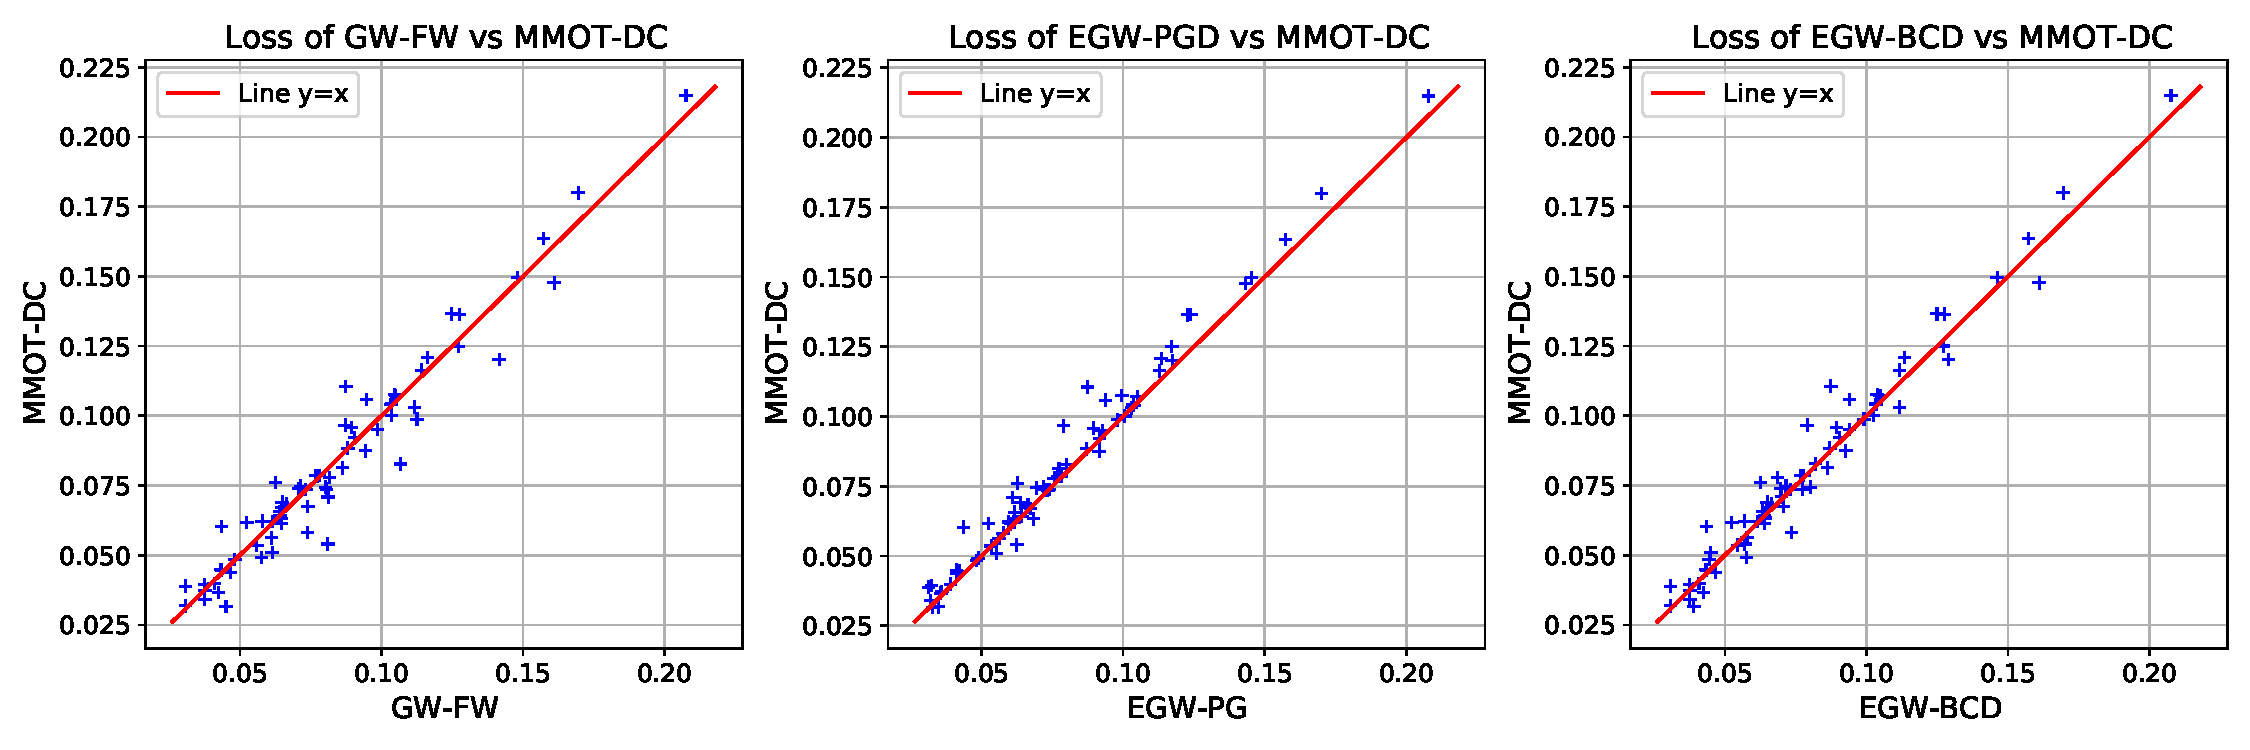
\includegraphics[width=\textwidth,height=\textheight,keepaspectratio]{./Chapitre2/fig/all_vs_MMOT-DC.pdf}
	\caption{Scatter plots of MMOT-DC versus other solvers. In all three plots, the points tend to concentrate around the line $y=x$,
  which indicates the comparable performance of MMOT-DC. On the other hand, the top-right plot shows the clear superiority of EGW-PGD.}
	\label{fig:gw}
\end{figure}
%%%%%%%%%%%%%%%%%%%%%%%%%%%%%%%%%%%%%%%

\paragraph{An empirical variation.} Intuitively, for sufficiently large $\varepsilon$, the minimisation of the KL divergence is prioritised
over the linear term in the objective function of the MMOT-DC problem, which implies that the optimal tensor $P^*$ is "close" to its
corresponding tensor product $P^*_{\# \mathcal T}$. So, instead of calculating the gradient at $P$, one may calculate at
$P_{\# \mathcal T}$. In this case, the gradient reads
\begin{equation*}
  \begin{split}
    \sum_{m=1}^M \nabla_P H_m(P_{\# \mathcal T}) =
    \big[ \log P_{\# \mathcal T_1} + P_{\# \mathcal T_1} \big] \oplus ... \oplus \big[ \log P_{\# \mathcal T_M} + P_{\# \mathcal T_M} \big],
  \end{split}
\end{equation*}
where $\oplus$ represents the tensor sum operator between two arbitrary-size tensors: $(A \oplus B)_{i,j}:= A_i + B_j$, where with some
abuse of notation, $i$ or $j$ can be understood as a tuple of indices. Thus, we avoid storing the $N$-D gradient tensor (as in the
algorithm \ref{algo:dc_MMOT}) and only need to store $M$ smaller-size tensors. Not only saving the memory,
this variation also seems to be empirically competitive with the original algorithm \ref{algo:dc_MMOT}, if not sometimes better,
in terms of COOT loss. The underlying reason might be related to the approximate DCA scheme \citep{Thanh15}, where one replaces both
steps in each DC iteration by their approximation. We leave the formal theoretical justification of this variation to the future work.
We call this variation \textit{MMOT-DC-v1} and use the same setup as in the experiment \ref{expe:2}.
\begin{figure}[ht]
  \centering
  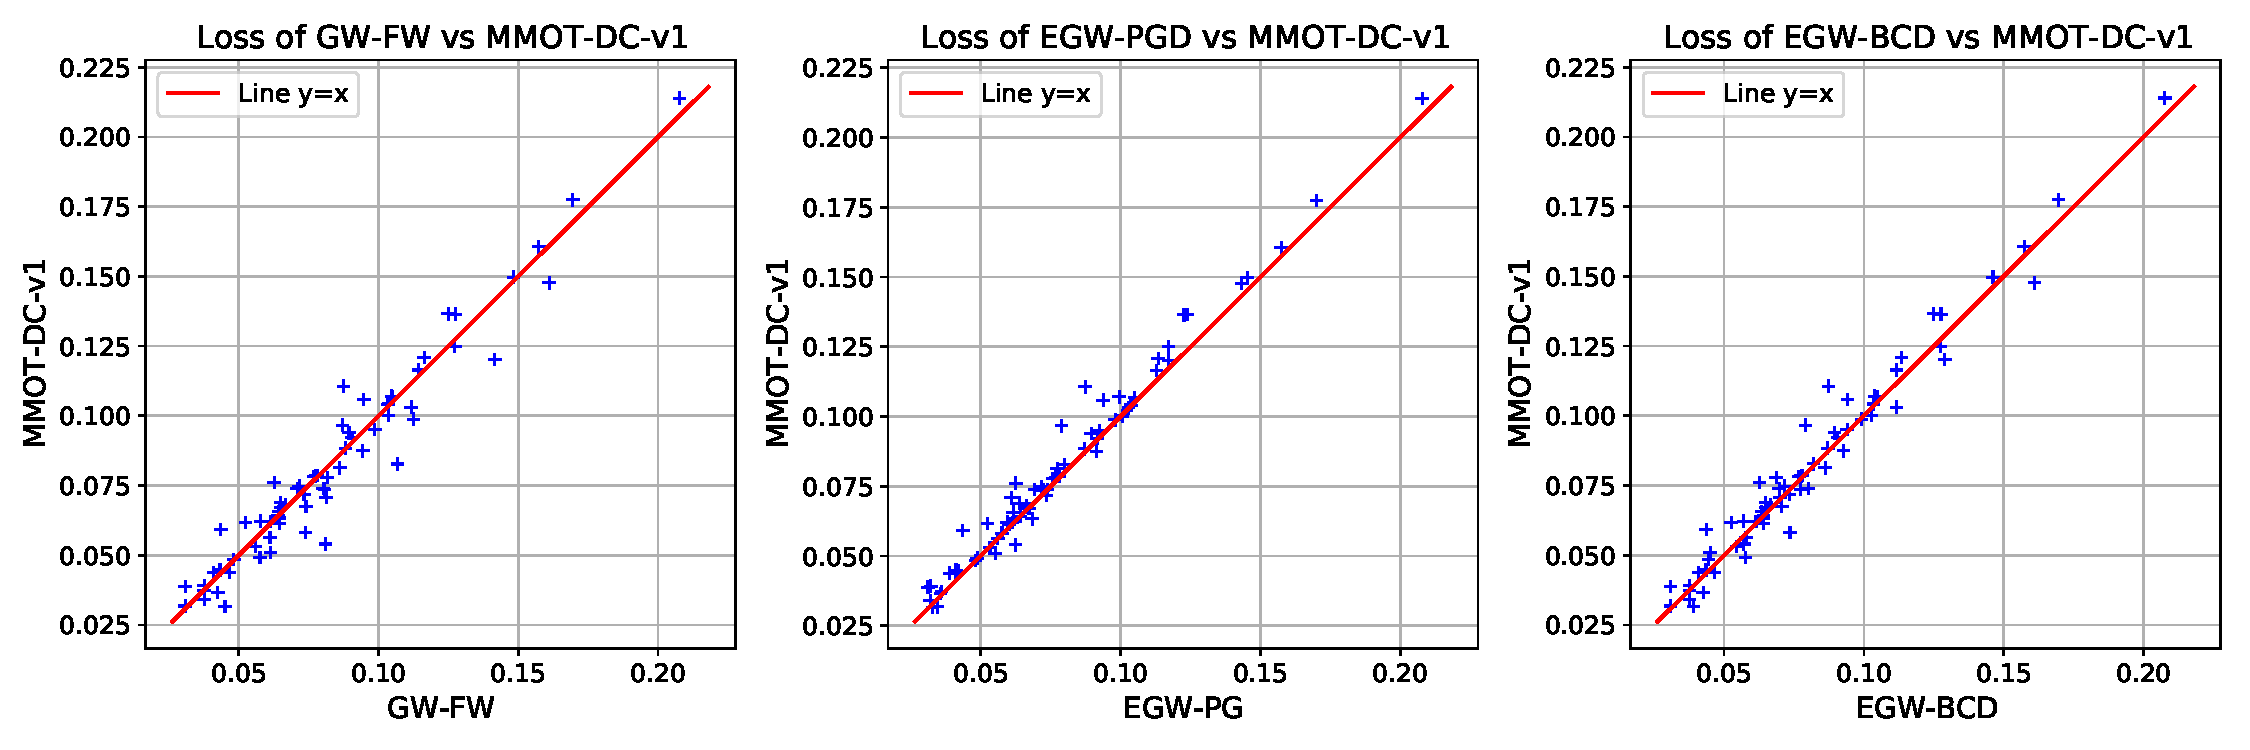
\includegraphics[width=\textwidth,height=\textheight,keepaspectratio]{./Chapitre2/fig/all_vs_MMOT-DC-v1.pdf}
  \caption{Scatter plots of MMOT-DC-v1 versus other solvers. In all three plots, the points tend to concentrate around the line $y=x$,
  which indicates the comparable performance of MMOT-DC-v1. On the other hand, the top-right plot shows the clear superiority of EGW-PGD.}
  \label{fig:coot_mmot_new}
\end{figure}

\begin{table}[H]
  \label{tab:coot_new}
  % \vskip 0.15in
  \begin{center}
    \begin{small}
      \begin{sc}
        \begin{tabular}{|c|c|}
          \hline
          MMOT-DC & MMOT-DC-v1 \\
          \hline
          0.0822 ($\pm$ 0.0364) & 0.0820 ($\pm$ 0.0361) \\
          \hline
        \end{tabular}
      \end{sc}
    \end{small}
  \end{center}
  \caption{Average and standard deviation of COOT loss of MMOT-DC and MMOT-DC-v1. The performance of the two algorithms is
  very similar.}
  % \vskip -0.1in
\end{table}

%%%%%%%%%%%%%%%%%%%%%%%%%%%%%%%%%%%%%%
\section{Continuous Co-Optimal Transport}
%%%%%%%%%%%%%%%%%%%%%%%%%%%%%%%%%%%%%%

\textbf{Important note:} \textit{this section is based on my unpublished working paper
on continuous COOT, its entropic regularization and unbalanced extension since November 2021.
It bears similarity with two concurrent works. More precisely, the continuous COOT
has also been first published by \citep{Chowdhury21b} in December 2021. Their work and ours
are based on the same mathematical framework, which results in the same metric property.
Apart from that, they pursue different research objectives, where
COOT is used to explore the categorical properties of the space of measure hypernetworks.}

\textit{Our study on the entropic COOT also shares some resemblance to
entropic GW distance in the paper of \citep{Zhang23} published in December 2022.
In particular, both of their analysis and ours rely on the block approximation technique
\citep{Carlier17} to show the convergence and quantify the approximation error,
and that ours can immediately extend to the GW setting. However, we consider different assumptions
on the mm-spaces, which result in the same convergence of minimizer and minimum,
but different upper bound of the approximation error.}

In this section, we present our unpublished work on the continuous COOT and its entropic approximation.
In particular, we will mostly follow the terminology and concepts of the published works
to avoid introducing unnecessary complication.

\subsection{From discrete to continuous Co-Optimal Transport}

\paragraph{Motivation and formulation} Recall that in GW distance,
by rewriting the measure networks $\cX = (X, c_X, \mu_X)$ and $\cY = (Y, c_Y, \mu_Y)$ as
$\widetilde{\cX} = ((X_1, \mu_1^X), (X_2, \mu_2^X), c_X)$ and
$\widetilde{\cY} = ((Y_1, \mu_1^Y), (Y_2, \mu_2^Y), c_Y)$, respectively, with
$X_1 = X_2 = X, Y_1 = Y_2 = Y$ and
$\mu_1^X = \mu^X_2 = \mu_X, \mu_1^Y = \mu^Y_2 = \mu_X$, one can reformulate the GW problem as
\begin{equation}
  \begin{split}
    \inf_{\pi_1, \pi_2}
    &\int_{X_1 \times Y_1} \int_{X_2 \times Y_2}
    \big\vert c_X(x_1, x_2) - c_Y(y_1, y_2) \big\vert^p \; d\pi_1(x_1, y_1) \; d\pi_2(x_2, y_2). \\
    \text{ subject to: } &\pi_k \in U(\mu_k^X, \mu_k^Y), \forall k = 1,2 \\
    &\pi_1 = \pi_2
  \end{split}
\end{equation}
When the equality constraint on the two couplings is relaxed,
we obtain a lower bound of the GW distance. Under this relaxation,
we can further allow that either $X_1 \neq X_2$ or $Y_1 \neq Y_2$.
The interest of such situation can be found, for example, in heterogenous domain adaptation,
where $X_1$ and $Y_1$ represent the "sample" spaces in the source and target domains, respectively,
and $X_2$ and $Y_2$ represent the "feature" spaces in the source and target domains, respectively.
As a result, the corresponding "sample" and "feature" couplings are also different in their natures.

\begin{definition}[Measure hypernetwork]
Suppose $(X_1, \mu_1^X)$ and $(X_2, \mu_2^X)$ are two Polish measure spaces,
and $c_X$ is a bounded measurable function on $X_1 \times X_2$.
We call the triplet $\cX = \big((X_1, \mu_1^X), (X_2, \mu_2^X), c_X \big)$
a \textbf{measure hypernetwork}. We also say $c_X$ is the \textbf{interaction}
between $X_1$ and $X_2$.
\end{definition}
With some abuse of notation and terminology, when $X_1 = X_2 = X$ and $\mu_1^X = \mu_2^X = \mu_X$,
we use measure hypernetwork and measure network (as in the context of GW) interchangeably.
When $X_1$ and $X_2$ are finite spaces (so $\mu_1^X$ and $\mu_2^X$ are histograms),
we say $\cX$ a finite measure hypernetwork. For convenience, we also refer the index $1$ as "sample"
and $2$ as "feature", for example, $X_1$ is the sample space, $\pi_2$ is the feature coupling.
\begin{definition}
  For $p \geq 1$, the COOT distance between two measure hypernetworks $\cX$ and $\cY$ is defined as
  \begin{align} \label{eq:cont_coot}
    \coot(\cX, \cY) =
    \inf_{\substack{\pi_1 \in U(\mu^X_1, \mu^Y_1) \\
    \pi_2 \in U(\mu^X_2, \mu^Y_2)}} \iint
    \big\vert c_X(x_1, x_2) - c_Y(y_1, y_2) \big\vert^p \; d\pi_1(x_1, y_1) \; d\pi_2(x_2, y_2).
  \end{align}
\end{definition}
It is not difficult to see that \Cref{eq:cont_coot} generalizes the discrete COOT \citep{Redko20}.
In practice, the input data is usually expressed as matrix,
whose rows represent samples and columns represent features.
In this case, the interaction value is precisely the coordinate of the data matrix.
On the other hand, the sample and feature spaces are unknown and have little interest and importance.

\begin{figure}[ht]
  \centering
  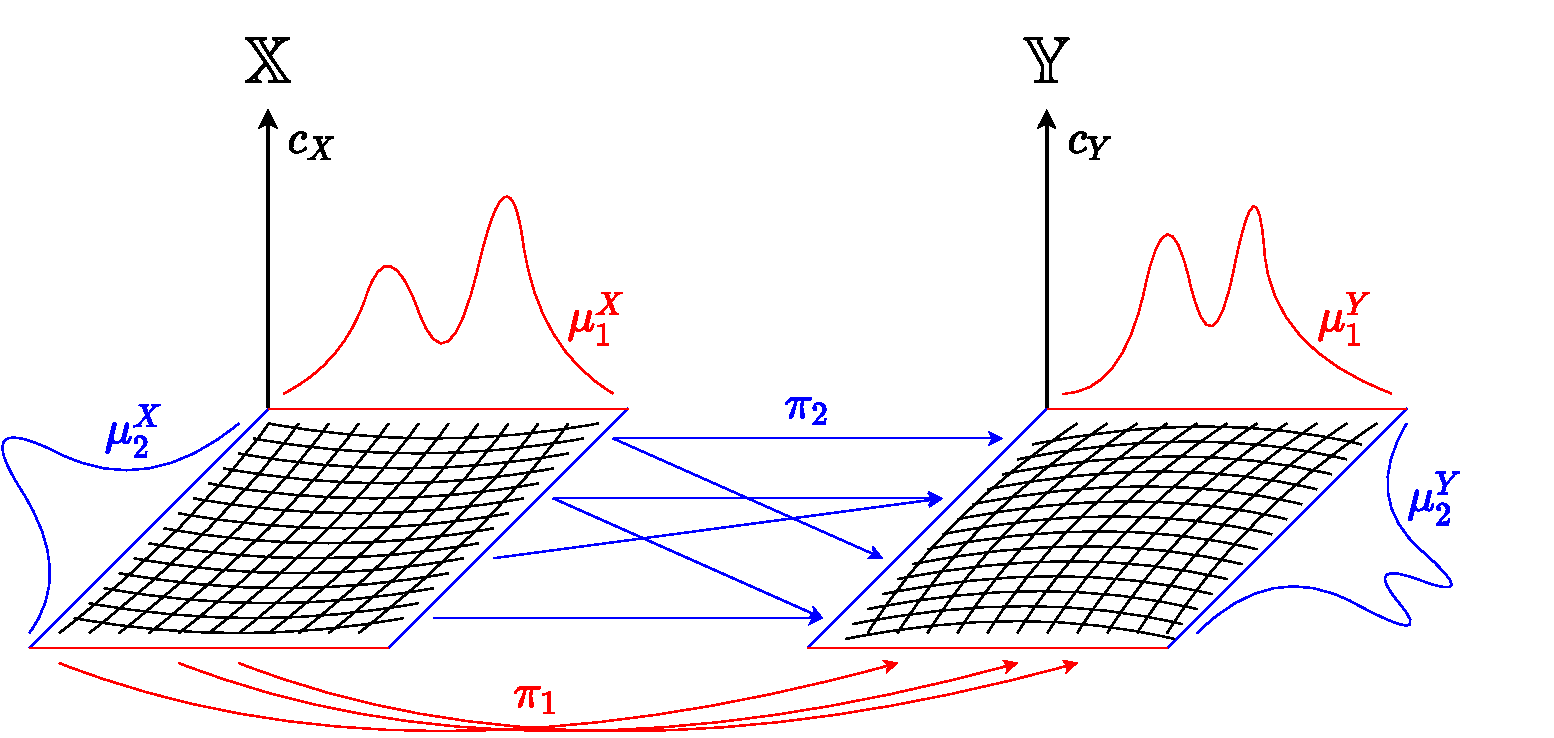
\includegraphics[width=0.9\textwidth, keepaspectratio]{./Chapitre2/fig/coot_diagram.pdf}
  \caption{Scatter plots of MMOT-DC-v1 versus other solvers. In all three plots, the points tend to concentrate around the line $y=x$,
  which indicates the comparable performance of MMOT-DC-v1. On the other hand, the top-right plot shows the clear superiority of EGW-PGD.}
  \label{fig:continuous_coot}
\end{figure}
\begin{proposition}
  \label{prop:exist_coot}
  The COOT problem always admits a minimizer.
\end{proposition}

%%%%%%%%%%%%%%%%%%%%%%%%%%%%%%%%%%%%%%%%%%
\subsection{Metric properties}
The framework on the isomorphism of GW distance presented in \Cref{subsec:prop_gw}
can be extended easily to COOT setting, or more generally, to the multi-coupling setting.
%%%%%%%%%%%%%%%%%%%%%%%%%%%%%%%%%%%%%%%%%
\begin{definition}[Relaxed mass splitting]
  A measure hypernetwork $\cZ$ is a \textbf{relaxed mass splitting} (RMS) of a
  measure hypernetwork $\cX$ if there exist two measure-preserving maps
  $\varphi_k: Z_k \to X_k$, for $k=1,2$, such that the pullback equality
  $c_Z = (\varphi_1, \varphi_2)^*c_X$ holds $\mu^Z_1 \otimes \mu_2^Z$-almost everywhere
  in $Z_1 \times Z_2$. We denote $\ms(\cX)$ the set of all mass splittings
  of $\cX$. This pair of maps $(\varphi_1, \varphi_2)$ is also called
  \textbf{basic weak isomorphism} in \citep{Chowdhury21b}.
\end{definition}
We denote $\rms(\cX)$ the set of all relaxed mass splittings of $\cX$. Clearly,
$\cX \in \rms(\cX)$, so $\rms(\cX)$ is not empty.
Moreover, in case of measure networks, if $\cZ \in \ms(\cX)$, then $\cZ \in \rms(\cX)$, meaning that
$\ms(\cX) \subset \rms(\cX)$. Now, we can define the isomorphism between the measure hypernetworks
as follows.
\begin{definition}[COOT-isomorphism] \label{coot_isomorphic}
  Two measure hypernetworks are
  \begin{enumerate}
    \item strongly isomorphic if there exist two \textbf{bijective}
    measure-preserving map from one hypernetwork to the other such that the pullback equality holds
    \textbf{everywhere}.
    \item semi-strongly isomorphic if one is the RMS of the other and vice versa.
    \item weakly isomorphic if they have a common RMS.
  \end{enumerate}
\end{definition}
This is an immediate relaxation of the isomorphism induced by the GW distance.
In particular, in case of measure networks, COOT-isomorphism is weaker:
isomorphism in GW sense implies COOT-isormorphism. The following result summarizes the relations
amongst the three types of COOT-isomorphism.
%%%%%%%%%%%%%%%%%%%%%%%%%%%%%%%%%%%%%%%%%%%%%%%%
\begin{corollary} \label{prop:strong_weak_iso}
  Given two measure hypernetworks $\cX$ and $\cY$. Consider three statements
  \begin{enumerate}
    \item[(1)] $\cX$ and $\cY$ are strongly isomorphism.
    \item[(2)] $\cX$ and $\cY$ are semi-strongly isomorphism.
    \item[(3)] $\cX$ and $\cY$ are weakly isomorphism.
  \end{enumerate}
  Then, the following relations hold
  \begin{enumerate}
    \item $(1) \implies (2) \implies (3)$.
    \item If $\cX$ and $\cY$ are finite, then $(2) \implies (1)$.
    \item If $\cX$ and $\cY$ are finite such that $|X_k| = |Y_k|$
    and $\mu_k^X, \mu_k^Y$ are uniform distributions, for $k = 1,2$, then
    $(3) \implies (2) \implies (1)$.
  \end{enumerate}
\end{corollary}
%%%%%%%%%%%%%%%%%%%%%%%%%%%%%%%%%%%%%%%%%%%%%%%%
We can also characterize the weak isomorphism by
\begin{proposition} \label{prop:coot_iso}
  Two measure hypernetworks $\cX$ and $\cY$ are COOT-weakly isomorphic if and only if
  $\coot(\cX, \cY) = 0$.
\end{proposition}
%%%%%%%%%%%%%%%%%%%%%%%%%%%%%%%%%%%%%%%%%%%%%%%%
\begin{proposition}[Theorem 1 in \citep{Chowdhury21b}] \label{prop:metric_prop}
  $\coot^{1/p}$ defines a metric on the space of measure hypernetworks, up to COOT-weak isomorphism.
\end{proposition}
%%%%%%%%%%%%%%%%%%%%%%%%%%%%%%%%%%%%%%%%%
\paragraph{Discussion on the setting of mm-space}
While the measure network fits in the COOT framework, this is usually not the case for
the mm-space since the distance function is only measurable in Polish space,
but not necessarily bounded. However, all previous results on the existence of minimizer and
metric property remain unchanged if one replaces measure hypernetworks by mm-spaces,
as long as COOT is finite. Moreover,
\begin{corollary}
For $p=2$, all types of COOT-isomorphisms are equivalent and
they are also equivalent with the isomorphism in GW sense.
\end{corollary}
This indicates that, similar to the GW distance, COOT can also be used to compare isometric objects,
for example objects transformed by reflection, rotation, translation or permutation.

%%%%%%%%%%%%%%%%%%%%%%%%%%%%%%%%%%%%%%%%%%%%%%%%
\subsection{Entropic regularization and approximation error}
%%%%%%%%%%%%%%%%%%%%%%%%%%%%%%%%%%%%%%%%%%%%%%%%
Similar to the Wasserstein and GW distances, entropic regularization can be used as a computationally
efficient approach to approximate the COOT. In this section,
we are interested in the following formulation of entropic COOT: for $\varepsilon > 0$,
\begin{align*}
  \coot_{\varepsilon} (\cX, \cY) =
  \inf_{\substack{\pi_1 \in U(\mu^X_1, \mu^Y_1) \\
  \pi_2 \in U(\mu^X_2, \mu^Y_2)}} &\int_{X_1 \times Y_1} \int_{X_2 \times Y_2}
  \big\vert c_X(x_1, x_2) - c_Y(y_1, y_2) \big\vert^p \; d\pi_1(x_1, y_1) \; d\pi_2(x_2, y_2) \\
  &+ \varepsilon \; \kl \big( \pi_1 \otimes \pi_2 \vert (\mu^X_1 \otimes \mu^Y_1) \otimes (\mu^X_2 \otimes \mu^Y_2) \big).
\end{align*}
This structure of the KL divergence term is particularly handy to prove all results related to
the entropic COOT. It can also be seen as a relaxation of the \textit{quadratic divergence}
\citep{Sejourne20} defined by $\kl^{\otimes 2}(\mu, \nu):= \kl(\mu \otimes \mu | \nu \otimes \nu)$,
which is used to define the unbalanced GW divergence. Note that, in the balanced setting,
the joint penalization in terms of KL divergence is in fact equivalent to the
independent penalization. Indeed, when $\pi_k \in U(\mu_k^X, \mu_k^Y)$, for $k=1,2$, we have
\begin{equation}
  \kl \big( \pi_1 \otimes \pi_2 \vert (\mu^X_1 \otimes \mu^Y_1) \otimes (\mu^X_2 \otimes \mu^Y_2) \big)
  = \kl(\pi_1 \vert \mu^X_1 \otimes \mu^Y_1) + \kl(\pi_2 \vert \mu^X_2 \otimes \mu^Y_2).
\end{equation}
In practical situations, since the couplings may not have the same nature (for example,
when working directly with the input data, rather than indirectly via the similarity matrix),
they can be regularized by different values of regularization.

\begin{proposition}
The entropic COOT problem always admits a minimizer.
\end{proposition}

\begin{assumption}
  \label{assump:ent_coot}
  The measure hypernetwork satisfies that sample and feature spaces are
  finite-dimensional vector spaces. The associated Borel probability measures
  have finite $p$-th moment, \textit{i.e.} $M_p(\mu) = \int ||x||^p \; d\mu(x) < \infty$, and are
  absolutely continuous with respect to the Lebesgue measure such that the negative entropy is finite,
  \textit{i.e.} $H(\mu) = \int \mu(x) \log(\mu(x)) \; dx < \infty$.
\end{assumption}
%%%%%%%%%%%%%%%%%%%%%%%%%%%%%%
\begin{proposition} \label{conv_ent_coot}
  Suppose that the measure hypernetworks $\cX, \cY$ satisfy \Cref{assump:ent_coot} and
  the interactions $c_X, c_Y$ are continuous. Then, $\coot_{\varepsilon}(\cX, \cY) \to \coot(\cX, \cY)$,
  when $\varepsilon \to 0$. Moreover, let $(\varepsilon_n)_{n \in \bbN}$ be a sequence of
  positive regularizations such that $\varepsilon_n \to 0$.
  Denote $\pi_n := (\pi_{1, n}, \pi_{2, n})$ the solution of the entropic problem
  $\coot_{\varepsilon_n} (\cX, \cY)$. Then, any cluster point of the sequence $(\pi_n)_n$ is
  a solution of the unregularized COOT problem.
\end{proposition}
%%%%%%%%%%%%%%%%%%%%%%%%%%%%%%
The above result is similar to the one known in entropic OT \citep{Carlier17}. This is due to the fact
that the entropic COOT can be reformulated as a variant of multi-marginal OT problem,
thus the block approximation and $\Gamma$-convergence techniques can be applied. Moreover,
similar to \citep{Genevay19}, when working with the bounded subsets in finite-dimensional vector spaces,
we can further quantify the approximation error.
%%%%%%%%%%%%%%%%%%%%%%%%%%%%%%
\begin{proposition} \label{prop:quant_bound_ent}
  Suppose $X_1, X_2$ are bounded subsets of $\bbR^{d_x}$ and
  $Y_1, Y_2$ are bounded subsets of $\bbR^{d_y}$,
  where $\diam(X_k), \diam(Y_k) \leq D$, for every $k=1,2$. Denote $d = \max(d_x, d_y)$.
  Suppose there exist two constants $q, L > 0$ such that
  $0 \leq c_X(x_1, x_2) \leq (L \vert\vert x_1 - x_2 \vert\vert)^q$,
  for every $(x_1,x_2) \in X_1 \times X_2$, and
  $0 \leq c_Y(y_1, y_2) \leq (L \vert\vert y_1 - y_2 \vert\vert)^q$,
  for every $(y_1,y_2) \in Y_1 \times Y_2$. Then, we have
  \begin{equation*}
    \coot_{\varepsilon}(\cX, \cY) - \coot(\cX, \cY) \leq \frac{2 d \varepsilon}{pq} +
    \frac{2d \varepsilon}{pq} \log\Big( \frac{pq (2DLd^{1/p})^{pq}}{2d \varepsilon} \Big).
  \end{equation*}
\end{proposition}
%%%%%%%%%%%%%%%%%%%%%%%%%
Let us consider two popular cases in practice: when $p=2$ and
\begin{itemize}
  \item[$\bullet$] $c_X$ and $c_Y$ are Euclidean distances (i.e. $q=L=1$), the bound becomes
  \begin{equation}
    d \varepsilon + d\varepsilon \log\Big( \frac{4D^2}{\varepsilon} \Big).
  \end{equation}

  \item[$\bullet$] $c_X$ and $c_Y$ are squared Euclidean distances (i.e. $q=2, L=1$),
  the bound becomes
  \begin{equation}
    \frac{d \varepsilon}{2} + \frac{d\varepsilon}{2} \log\Big( \frac{32dD^4}{\varepsilon} \Big).
  \end{equation}
\end{itemize}
In both cases, the dependence of the bound on the maximal distance $D$ between points
within each space (even only at logarithmic scale) and on the dimension $d$ indicates
that either high dimensional space, or large intra-space distance (for example, due to outliers)
can have negative impact on the approximation error. On the other hand,
by comparing these two bounds, we deduce that if $\log(2d \varepsilon) \leq 1$,
then the squared Euclidean distances generates a provably better (smaller) upper bound.

With little modification of the proof, exactly the same upper bound in \Cref{prop:quant_bound_ent}
remains true for GW distance. We note that \citep{Zhang23} also establish the
approximation error between unregularized and entropic GW, but they rely on different assumptions
to ours. In particular, their result only holds for $2$-GW distance,
when the distance function is the squared-Euclidean norm. By contrast,
\Cref{prop:quant_bound_ent} holds for any $p$-GW distance and any $L^q$-norm as distance function.

%%%%%%%%%%%%%%%%%%%%%%%%%%%%%%%%%%%%%%
\section{Conclusion and future work}
%%%%%%%%%%%%%%%%%%%%%%%%%%%%%%%%%%%%%%

\subsection{Stability of Co-Optimal Transport}

COOT setting: given two sample-feature spaces
$\mathcal X_1 = ((X_1^s, \mu_1^s), (X_1^f, \mu_1^f), \xi_1)$ and
$\mathcal X_2 = ((X_2^s, \mu_2^s), (X_2^f, \mu_2^f), \xi_2)$. COOT reads
\begin{equation*}
    \coot(\mathcal X_1, \mathcal X_2) =
    \inf_{\substack{\pi^s \in U() \\ \pi^f \in U()}}
    \int |\xi_1 - \xi_2|^2 d\pi^s d\pi^f
\end{equation*}
Consider the "semi-empirical" spaces:
$\widehat{\mathcal X}_i := ((\widehat{X}_i^s, \widehat{\mu}_i^s), (X_i^f, \mu_i^f), \xi_i))$, where
we fix the dimension $f$ and only consider the empirical version of sample measures.
Now, how does the feature coupling behave when $\widehat{\mu}^s \to \mu^s$?, i.e. when $n \to \infty$,
quantify
\begin{equation}
    | \coot(\mathcal X_1, \mathcal X_2) -
    \coot(\widehat{\mathcal X}_1, \widehat{\mathcal X}_2) |
\end{equation}
We can first start with finite-dimensional feature spaces (so the feature coupling is a matrix).

\subsection{Sample complexity of Co-Optimal Transport and GW distance}
